% Author: Alfredo Sánchez Alberca (email:asalber@ceu.es)
% Plot with the phases of the statistical cycle
\begin{tikzpicture}[every label/.style={text=color1}]
\tikzstyle{arrow} = [-latex, color1, line width=12pt];
\tikzstyle{node} = [align=center, inner sep=10pt];
\node[node, label=-90:Población] (population) at (1,1)
{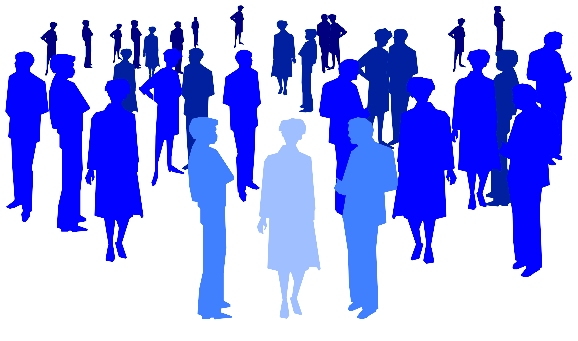
\includegraphics[height=1.5cm]{img/introduccion/poblacion}}; 
\pause
\node[node,label=90:Muestra] (sample) at
(1,6){
\includegraphics[height=1.5cm]{img/introduccion/muestra.png}}; 
\node at (1,3.4) [fill=color1,single arrow,shape border rotate=90,text=white, minimum width=1.2cm, minimum
height=3cm]{
\rotatebox{90}{Muestreo}\phantom{}};
\pause
\node[node,label=90:Resumen estadístico] (statistics) at (8,6) {\Large $\bar x$ \quad $s^2$\\\Large \quad $p$ \quad
$g_1$}; 
\node at (4.5,6) [fill=color1,single arrow,shape border rotate=0,text=white, minimum width=1.2cm, minimum
height=3cm]{
Estadística Descriptiva\phantom{}};
\pause
\node[node,label=-90:Modelo] (model) at (8,1) {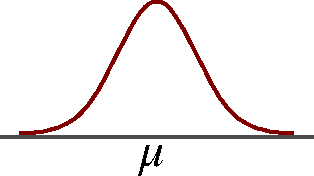
\includegraphics[scale=0.5]{img/introduccion/normal}};
\node at (8,3.6) [fill=color1,single arrow,shape border rotate=270,text=white, minimum width=1.2cm, minimum
height=3cm]{
\rotatebox{90}{Est. Inferencial}\phantom{}};
\pause
\node at (4.5,1) [fill=color1,single arrow,shape border rotate=180,text=white, minimum width=1.2cm, minimum
height=3cm]{ Predicción\phantom{}};
\end{tikzpicture}